
\documentclass{beamer}
\usecolortheme{dove}
\setbeamertemplate{navigation symbols}{}
\usepackage{amsmath,amssymb,amsfonts,amsthm, multicol, subfigure, color}
\usepackage{bm}
\usepackage{graphicx}
\usepackage{tabularx}
\usepackage{booktabs}
\usepackage{hyperref}
\usepackage{pdfpages}
\usepackage{xcolor}
\definecolor{seagreen}{RGB}{46, 139, 87}
\def\independenT#1#2{\mathrel{\rlap{$#1#2$}\mkern2mu{#1#2}}}
\newcommand\indep{\protect\mathpalette{\protect\independenT}{\perp}}
\def\log{\text{log}}
\newcommand\logit{\text{logit}}
\newcommand\iid{\stackrel{\text{iid}}{\sim}}
\newcommand\E{\text{E}}
\newcommand\V{\text{V}}
\renewcommand\P{\text{P}}
\newcommand{\Cov}{\text{Cov}}
\newcommand{\Cor}{\text{Cor}}
\newcommand\doop{\texttt{do}}
\usepackage{stackrel}
\usepackage{tikz}
\usetikzlibrary{arrows,shapes.arrows,positioning,shapes,patterns,calc}
\newcommand\slideref[1]{\vskip .1cm \tiny \textcolor{gray}{{#1}}}
\newcommand\red[1]{\color{red}#1}
\newcommand\blue[1]{\color{blue}#1}
\newcommand\gray[1]{\color{gray}#1}
\newcommand\seagreen[1]{\color{seagreen}#1}
\newcommand\purple[1]{\color{purple}#1}
\newcommand\orange[1]{\color{orange}#1}
\newcommand\black[1]{\color{black}#1}
\newcommand\white[1]{\color{white}#1}
\newcommand\teal[1]{\color{teal}#1}
\newcommand\magenta[1]{\color{magenta}#1}
\newcommand\Fuchsia[1]{\color{Fuchsia}#1}
\newcommand\BlueGreen[1]{\color{BlueGreen}#1}
\newcommand\bblue[1]{\textcolor{blue}{\textbf{#1}}}
\newcommand\bred[1]{\textcolor{red}{\textbf{#1}}}
\newcommand\bgray[1]{\textcolor{gray}{\textbf{#1}}}
\newcommand\bgreen[1]{\textcolor{seagreen}{\textbf{#1}}}
\newcommand\bref[2]{\href{#1}{\color{blue}{#2}}}
\colorlet{lightgray}{gray!40}
\pgfdeclarelayer{bg}    % declare background layer for tikz
\pgfsetlayers{bg,main} % order layers for tikz
\newcommand\mycite[1]{\begin{scriptsize}\textcolor{darkgray}{(#1)}\end{scriptsize}}
\newcommand{\tcframe}{\frame{
%\small{
\only<1|handout:0>{\tableofcontents}
\only<2|handout:1>{\tableofcontents[currentsubsection]}}
%}
}

\usepackage[round]{natbib}
\bibliographystyle{humannat-mod}
\setbeamertemplate{enumerate items}[default]
\usepackage{mathtools}
\usepackage{ulem}
\usepackage{cancel}

% Need to add examples

\newcommand{\goalsframe}{\begin{frame}{Learning goals for today}
At the end of class, you will be able to:
\begin{enumerate}
\item Reason about when future treatments can proxy for unmeasured confounding
\end{enumerate} \vskip .2in
Note that this class is based on: \vskip .1in
Elwert, F., \& Pfeffer, F. T. (2022). \bref{https://doi.org/10.1177/0049124119875958}{The future strikes back: Using future treatments to detect and reduce hidden bias.} \textit{Sociological Methods \& Research}, 51(3), 1014-1051.
\end{frame}}

\title{25. Future treatments as proxies for confounding\vskip .1in Class guest: Felix Elwert\\University of Wisconsin, Madison}
\author{Ian Lundberg\\Cornell Info 6751: Causal Inference in Observational Settings\\Fall 2022}
\date{17 Nov 2022}

\begin{document}

\maketitle

\goalsframe

\begin{frame}
\Large
A few things we've recently covered

\end{frame}

\begin{frame}
\begin{tikzpicture}[x = \textwidth, y = .9\textheight]
\node at (0,0) {};
\node at (1,1) {};
\only<1-3>{
\node[anchor = north west] at (0,.9) {\includegraphics[height = .8\textheight]{figures/hc_fig2}};
\node[anchor = north] at (.2,1) {Hern\'an \& Cole 2009};
}
\only<2>{
\node (a) at (.7, .5) {$A$};
\node (l) at (.8, .6) {$L$};
\node (y) at (.9, .5) {$Y$};
\node (ltilde) at (.8, .7) {$\tilde{L}$};
\draw[->, thick] (a) -- (y);
\draw[->, thick] (l) -- (y);
\draw[->, thick] (l) -- (a);
\draw[->, thick] (l) -- (ltilde);
}
\only<3->{
\node[anchor = north] at (.8,1) {Elwert \& Pfeffer~2022};
\node[anchor = north east] at (1,.9) {\includegraphics[width = .4\textwidth]{figures/ep_fig1}};
}
\node<4-5>[anchor = north west] at (0,.9) {If you measure $U$};
\node<4-5>[anchor = north west] at (0,.8) {$\E(Y\mid A,U) = \alpha + \beta A + \gamma U$};
\node<5>[anchor = north west, font = \footnotesize, align = left] at (0, .65) {$\begin{aligned}
\beta &= \frac{\Cov(T,Y) - \Cov(U,Y)\Cov(U,A)}{1 - \left[\Cov(U,A)\right]^2} \\ 
&= \frac{\big(b + ac\big) - \big((c + ab)a\big)}{1 - a^2} \\ 
&= \frac{b + ac - ac - a^2b}{1 - a^2} \\ 
&= \frac{b(1 - a^2)}{1 - a^2}\\ 
&= b
\end{aligned}$};
\node<6->[anchor = north west] at (0,.9) {If you don't measure $U$};
\node<7->[anchor = north west] at (0,.8) {$\E(Y\mid A,F) = \alpha + \beta A + \gamma F$};
\node<8>[anchor = south west, font = \footnotesize] at (0,0) {$\begin{aligned}
\beta &= \frac{\Cov(A,Y) - \Cov(\tilde{L},Y)\Cov(\tilde{L},A)}{1 - \left[\Cov(\tilde{L},A)\right]^2} \\ \pause
&= \frac{\big(b + ac\big) - \big((cd + abd)ad\big)}{1 - a^2d^2} \\ \pause
&= \frac{b + ac - acd^2 - a^2bd^2}{1 - a^2d^2} \\ \pause
&= \frac{b(1 - a^2d^2) + ac(1 - d^2)}{1 - a^2d^2} \\ \pause
&= b + \underbrace{ac}_{\substack{\text{Bias}\\\text{without}\\\text{control}}}\underbrace{\frac{1 - d^2}{1 - a^2d^2}}_{\substack{\text{Bias}\\\text{Multiplier}\\\lvert M \rvert <1}} \\
\end{aligned}$};
\node<9->[anchor = north west] at (0,.3) {Control Estimator};
\node<9->[anchor = south west, font = \footnotesize] at (0,0) {$\begin{aligned}
\beta &= b + \underbrace{ac}_{\substack{\text{Bias}\\\text{without}\\\text{control}}}\underbrace{\frac{1 - d^2}{1 - a^2d^2}}_{\substack{\text{Bias}\\\text{Multiplier}\\\lvert M \rvert <1}} \\
\end{aligned}$};
\node<10->[anchor = north west] at (.5,.3) {Difference (Mayer) Estimator};
\node<10->[anchor = south west, font = \footnotesize] at (.5,0) {$\begin{aligned}
\beta - \gamma &= b + \underbrace{ac}_{\substack{\text{Bias}\\\text{without}\\\text{control}}}\underbrace{\frac{a - d}{a - a^2d}}_{\substack{\text{Bias}\\\text{Multiplier}\\\lvert M \rvert}} \\
\end{aligned}$};
\node<11->[anchor = west] at (0,.5) {\includegraphics[width = .4\textwidth]{figures/ep_fig3}};
\end{tikzpicture}
\end{frame}

\begin{frame}
\Large
Parts of the paper we have not yet covered

\end{frame}

\begin{frame}{Empirical example}
What is the effect of log parental income on years of education? \vskip .2in
\begin{center}
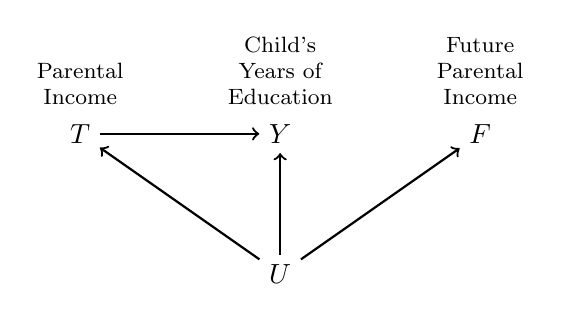
\begin{tikzpicture}[x = 1in, y = .7in]
\node (t) at (0,0) {$T$};
\node (y) at (1,0) {$Y$};
\node (f) at (2,0) {$F$};
\node (u) at (1,-1) {$U$};
\draw[->, thick] (t) -- (y);
\draw[->, thick] (u) -- (t);
\draw[->, thick] (u) -- (y);
\draw[->, thick] (u) -- (f);
\node[anchor = south, align = center, font = \footnotesize] at (t.north) {Parental\\Income};
\node[anchor = south, align = center, font = \footnotesize] at (y.north) {Child's\\Years of\\Education};
\node[anchor = south, align = center, font = \footnotesize] at (f.north) {Future\\Parental\\Income};
\end{tikzpicture}
\end{center}
Panel Study of Income Dynamics. Born 1956--1968. ($n = 1,513$)
\begin{itemize}
\item $T$ log family income averaged at child age 13--17
\item $Y$ years of education by age 24
\item $F$ log family income at child age 25--29 
\end{itemize}
\end{frame}

\begin{frame}

\includegraphics[width = \textwidth]{figures/ep_table3}

\end{frame}

\begin{frame}

\includegraphics[width = \textwidth]{figures/ep_fig4}

\end{frame}

\begin{frame}{Challenge 1: True State Dependence}
\includegraphics[width = .4\textwidth]{figures/ep_fig5}
\end{frame}

\begin{frame}{Challenge 2: Confounded True State Dependence}
\includegraphics[width = .4\textwidth]{figures/ep_fig6}
\end{frame}

\begin{frame}{Challenge 3: Unconfounded Study with Selection}
\includegraphics[width = .4\textwidth]{figures/ep_fig7}
\end{frame}

\begin{frame}{Challenge 4: Confounded Study with Selection}
\includegraphics[width = .4\textwidth]{figures/ep_fig8}\only<2->{\vskip .2in
\includegraphics[width = \textwidth]{figures/ep_table2}}
\end{frame}

\begin{frame}{Nonparametric results}

Previous results relied on a linear path model.\\
Next results rely only on a DAG (nonparametric). \vskip .3in \pause
Motivating (but incomplete) intuition:\vskip .1in
\begin{quote}
A future treatment $F$ cannot affect an outcome $Y$.\vskip .1in
If the outcome $Y$ is related to $F$,\\then there must be unobserved confounding.
\end{quote}
\end{frame}

\begin{frame}{Nonparametric Example 1.}{Does a relationship between $Y$ and $F$ imply confounding?} \vskip .1in
Is $F$ related to $Y$? \only<2->{\hfill Yes. $Y\leftarrow U\rightarrow F$}\\
Is $T\rightarrow Y$ confounded given $X$? \only<3->{\hfill Yes. $T\leftarrow V\rightarrow \boxed{X}\leftarrow U\rightarrow Y$}
\begin{center}
\includegraphics[width = .5\textwidth]{figures/ep_fig9}
\end{center}
\onslide<4->{
%All assumptions hold.\\
A conditional relationship between $Y$ and $F$ implies confounding.
%$$F\cancel\indep Y \mid \{T,X\} \qquad \rightarrow \qquad \{Y^0,Y^1\}\cancel\indep T\mid X$$ \vskip .2in
}
\end{frame}

\begin{frame}{Nonparametric results: Example 2.}{Does a relationship between $Y$ and $F$ imply confounding?} \vskip .1in
Is $F$ related to $Y$? \only<2->{\hfill Yes. $Y\leftarrow V\rightarrow F$}\\
Is $T\rightarrow Y$ confounded? \only<3->{\hfill No.}

\begin{center}
\includegraphics[width = .5\textwidth]{figures/ep_fig10}
\end{center}
\onslide<4->{
A conditional relationship between $Y$ and $F$ does not imply confounding.
%$$F\cancel\indep Y \mid \{T,X\} \qquad \cancel\rightarrow \qquad \{Y^0,Y^1\}\cancel\indep T\mid X$$ \vskip .2in
}
\end{frame}

\begin{frame}{Nonparametric results: Example 3.}{Does a relationship between $Y$ and $F$ imply confounding?} \vskip .1in
Is $F$ related to $Y$? \only<2->{\hfill Yes. $Y\leftarrow V\rightarrow F$}\\
Is $T\rightarrow Y$ confounded? \only<3->{\hfill No.}

\begin{center}
\includegraphics[width = .5\textwidth]{figures/ep_fig11}
\end{center}
\onslide<4->{
A conditional relationship between $Y$ and $F$ does not imply confounding.
%$$F\cancel\indep Y \mid \{T,X\} \qquad \cancel\rightarrow \qquad \{Y^0,Y^1\}\cancel\indep T\mid X$$ \vskip .2in
}
\end{frame}

\begin{frame}{Two nonparametric results: A formal answer}{What does the relationship between $F$ and $Y$ tell us about confounding?} \pause
\begin{tikzpicture}[x = \textwidth, y = .8\textheight]
\node at (0,0) {};
\node at (1,1) {};
\node (x) at (.6, .95) {$X$};
\node (t) at (.7, .95) {$T$};
\node (y) at (.8, .95) {$Y$};
\node (f) at (.9, .95) {$F$};
\node (v) at (.8, .83) {$V$};
\draw[->, thick] (t) -- (y);
\draw[->, thick] (v) -- (t);
\draw[->, thick] (v) -- (f);
\draw[->, thick] (v) -- (y);
\draw[->, thick] (x) -- (t);
\draw[->, thick] (x) to[bend left] (f);
\draw[->, thick] (x) to[bend left] (y);
\draw[->, thick] (x) to[bend right] (v);
\node[anchor = north west] at (0,.85) {Result 11. (Requires Assumption 1)};
\node[anchor = north] at (.5,.75) {$F\indep Y \mid \{T,X\} \qquad \rightarrow \qquad \{Y^0,Y^1\}\indep T\mid X$};
\node[anchor = north west] at (0,.65) {Result 12. (Requires Assumptions 1--3)};
\node[anchor = north] at (.5, .55) {$F\cancel\indep Y \mid \{T,X\} \qquad \rightarrow \qquad \{Y^0,Y^1\}\cancel\indep T\mid X$};
\node[anchor = north west, align = left] (asm1) at (0,.4) {Assumption 1. There exists some unobserved $V$ such that\\\phantom{Assumption 1. }$V\rightarrow T$ and $V\cancel\indep F\mid \{T,X\}$};
\node[anchor = north west] (asm2) at (asm1.south west) {Assumption 2. All unobserved causes of $F$ also cause $T$};
\node[anchor = north west] at (asm2.south west) {Assumption 3. $Y$ does not directly or indirectly cause $F$};
\end{tikzpicture}
\end{frame}

\begin{frame}{Discussion: Applied examples}

The usefulness of future treatments relies heavily on this DAG.

\begin{center}
\includegraphics[width = .4\textwidth]{figures/ep_fig1}
\end{center}

\bgray{Exercise.} Discuss the plausibility of this DAG in applied cases.\vskip .1in
\bref{https://tinyurl.com/FutureTreatmentsExamples}{tinyurl.com/FutureTreatmentsExamples}

\end{frame}

\begin{frame}{Group \only<1>{1}\only<2>{2}\only<3>{3}\only<4>{4}}
\begin{center}
\begin{tikzpicture}[x = 1.2in, y = .9in]
\node (t) at (0,0) {$T$};
\node (y) at (1,0) {$Y$};
\node (f) at (2,0) {$F$};
\node (u) at (1,-1) {$U$};
\draw[->, thick] (t) -- (y);
\draw[->, thick] (u) -- (t);
\draw[->, thick] (u) -- (y);
\draw[->, thick] (u) -- (f);
\only<1>{
\node[anchor = south, align = center, font = \footnotesize] at (t.north) {Image in\\Tweet\\on Dec 1};
\node[anchor = south, align = center, font = \footnotesize] at (y.north) {Retweets\\by Dec 7};
\node[anchor = south, align = center, font = \footnotesize] at (f.north) {Image in\\Tweet\\after Dec 7};
\node[anchor = north, align = center, font = \footnotesize] at (u.south) {Author\\skill};
}
\only<2>{
\node[anchor = south, align = center, font = \footnotesize] at (t.north) {Child visits\\public library\\in August};
\node[anchor = south, align = center, font = \footnotesize] at (y.north) {Child excited\\about school\\in September};
\node[anchor = south, align = center, font = \footnotesize] at (f.north) {Child visits\\public library\\in October};
\node[anchor = north, align = center, font = \footnotesize] at (u.south) {Child\\enjoys\\learning};
}
\only<3>{
\node[anchor = south, align = center, font = \footnotesize] at (t.north) {Workers\\strike};
\node[anchor = south, align = center, font = \footnotesize] at (y.north) {Pay\\rises};
\node[anchor = south, align = center, font = \footnotesize] at (f.north) {Workers\\strike\\next year};
\node[anchor = north, align = center, font = \footnotesize] at (u.south) {Adversarial\\managerial\\culture};
}
\only<4>{
\node[anchor = south, align = center, font = \footnotesize] at (t.north) {Neighborhood has\\vacant housing\\units};
\node[anchor = south, align = center, font = \footnotesize] at (y.north) {Crime\\rate};
\node[anchor = south, align = center, font = \footnotesize] at (f.north) {Future\\vacant\\units};
\node[anchor = north, align = center, font = \footnotesize] at (u.south) {Local\\economic\\difficulties};
}
\end{tikzpicture}
\end{center}
\end{frame}

\goalsframe

\begin{frame}{Let me know what you are thinking}

\begin{huge} \bref{https://tinyurl.com/CausalQuestions}{tinyurl.com/CausalQuestions} \end{huge}
\vskip .7in

Office hours TTh 11am-12pm and at \bref{https://calendly.com/ianlundberg/office-hours}{calendly.com/ianlundberg/office-hours}\\Come say hi!

\end{frame}


\end{document}
